\documentclass{article}
% \usepackage{corl_2022} % Use this for the initial submission.
\usepackage[final]{corl_2022} % Uncomment for the camera-ready ``final'' version.
\usepackage{times} % assumes new font selection scheme installed
\usepackage{brian}
\graphicspath{{../images/}}
\usepackage[export]{adjustbox}
\usepackage{wrapfig}
\usepackage{xcolor}
% \usepackage{biblatex}

% Bibliography
% \usepackage[style=ieee,doi=false,isbn=false,url=false,eprint=false]{biblatex}
% \AtEveryBibitem{\clearlist{language}}  % remove language field from bib entries
% \addbibresource{references.bib}
% \renewcommand*{\bibfont}{\small}


\title{
  % JDMD: Leveraging Analytic Jacobians to Quickly Learn Effective MPC Controllers
  % JDMD: A Sample-Efficient Method for Learning How To Control Nonlinear Systems
  % JDMD: Boosting Sample Efficiency in Bilinear Koopman Models through Derivative Information
  % JDMD: Quickly Boost MPC Performance via Koopman Operators and Approximate Derivatives
  % JDMD: Adapting Adapting Extended Dynamic Mode Decomposition to Leverage What You Know 
  JDMD: Extended Dynamic Mode Decomposition with Jacobian Residual Penalization
  for Learning Bilinear, Control-affine Koopman Models
}

\author{
Brian E. Jackson \\
Robotics Institute \\
Carnegie Mellon University \\
\texttt{brianjackson@cmu.edu} \\
\and
Jeong Hun Lee \\
Robotics Institute \\
Carnegie Mellon University \\
\texttt{jeonghunlee@cmu.edu} \\
\and
Kevin Tracy \\
Robotics Institute \\
Carnegie Mellon University \\
\texttt{ktracy@cmu.edu} \\
\and
Zachary Manchester \\
Robotics Institute \\
Carnegie Mellon University \\
\texttt{zacm@cmu.edu} \\
}

\begin{document}
\maketitle

\begin{abstract}
  % Combining the benefits of data-driven and model-based control techniques for nonlinear
  % dynamics systems has many potential advantages. Compared to purely data-driven approaches,
  % this could include benefits such as increasing sampling efficiency, reducing training
  % time, or increasing generalization. For purely model-based approaches such as
  % model-predictive control, this could in- crease robustness to model uncertainty or improve
  % overall performance by adapt- ing the controller based on observations from the real
  % system. 
  We present a novel extension to previous data-driven approaches based on Koopman
  operator theory that combines many of the benefits of model-based and data-driven
  approaches.  By including derivative information from an approximate analytical model, we
  show that we can quickly learn an efficient bilinear representation of the system
  dynamics, that, when combined with a novel linear MPC method that projects the dynamics
  into the original state space, offers performance improvements over nominal linear MPC
  with just a few training trajectories. We demonstrate increased sampling efficiency,
  increased generalization, and robustness to training hyperparameters compared to previous
  approaches
\end{abstract}

\section{Introduction}

Controlling complex, underactuated, and highly nonlinear autonomous systems remains an
active area of research in robotics, despite decades of previous work exploring
effective algorithms and the development of substantial theoretical analysis. Classical
approaches typically rely on local linear approximations of the nonlinear system, which
are then used in any of a multitude of linear control techniques, such as PID, pole
placement, Bode analysis, H-infinity, LQR, or linear MPC.  These approaches only work
well if the states of the system always remain close to the equilibrium point or
reference trajectory about which the system was linearized. The region for which these
linearizations remain valid can be extremely small for highly nonlinear systems.
Alternatively, model-based methods for nonlinear optimal control have shown great
success, as long as the model is well known and an accurate estimate of the global state
can be provided. These model-based techniques leverage decades of insight into
dynamical systems and have demonstrated incredible performance on complicated
autonomous systems 
\cite{Farshidian2017,Kuindersma2014,Bjelonic2021,Subosits2019} . On the
other hand, data-driven techniques such as reinforcement learning have received
tremendous attention over the last decade and have begun to demonstrate impressive
performance and robustness for complicated robotic systems in unstructured environments
\cite{Karnchanachari2020,Hoeller2020,Li2021}. While these approaches are attractive
since they require little to no previous knowledge about the system, they often require
large amounts of data and fail to generalize outside of the domain or task on which they
were ``trained.''

In this work we propose a novel method that combines the benefits of model-based and
data-driven methods, based on recent work  applying Koopman Operator Theory to
controlled dynamical systems 
\cite{Meduri2022,Bruder2021,Korda2018,Folkestad2020,Suh2020}.
% \cite{Meduri2022,Bruder2021, Korda2021}
% \cite{Meduri2022, Folkestad2021, Bruder2021, Korda2018, Folkestad2020a, Folkestad2020b}.  
By leveraging data collected from an
unknown dynamical system along with derivative information from an approximate
analytical model, we can efficiently learn a bilinear representation of the system
dynamics that performs well when used in traditional model-based control techniques such
as linear MPC. By leveraging information from an analytical model, we can dramatically
reduce the number of samples required to learn a good approximation of the true
nonlinear dynamics. We also show the effectiveness of linear MPC on these systems 
when the learned bilinear system is linearized and projected back into the original 
state space. The result is a fast, robust, and sample-efficient pipeline for quickly 
learning a model that beats previous Koopman-based linear MPC approaches as well as 
purely model-based linear MPC controllers that do not leverage data collected from the 
actual system. To learn these bilinear representations, we also propose 
a numerical technique that allows for large systems to be trained while limiting the 
peak memory required to solve the least-squares problem.

The current work is most closely related to recent work out of Caltech 
\cite{Folkestad2020,Folkestad2021,Folkestad2021a} which learn a bilinear
model and apply nonlinear model-predictive control directly on the learned bilinear 
dynamics. Similarly, control Lyapunov functions were also recently used directly on the 
learned bilinear dynamics \cite{Narasingam2022}. These works build on a foundational paper
applying MPC to nonlinear systems using Koopman operators to learn a linear model directly
\cite{Korda2018}.

In summary, our contributions are:
\begin{itemize}
  \item A novel extension to extended dynamic mode decomposition (eDMD) that
  incorporates gradient information from an approximate analytic model;
  
  \item a simple linear MPC control technique for learned bilinear control systems
  that is computationally efficient online, which, when combined with the proposed
  extension to eDMD, requires extremely little training data to get a good control
  policy; and
  
  \item a recursive, batch QR algorithm solving the least-squares problems that arise 
  when learning bilinear dynamical systems using eDMD.
\end{itemize}

The paper is organized as follows: in Section \ref{sec:Preliminaries/Background} we 
give some background on the application of Koopman operator theory to controlled 
dynamical systems and review some related works. Section \ref{sec:jdmd} describes
the proposed algorithm for combining data-driven and model-based approaches, while 
\ref{sec:projected_mpc} proposed an efficient technique for controlling these learned models
online. In Section \ref{sec:rls} we outline an memory-efficient technique for solving the 
large, sparse linear least-squares problems that arise when applying the proposed adaption 
to eDMD. Lastly, Section \ref{sec:results} provides numerical analysis of the 
proposed algorithm, applied to a simulated cartpole, quadrotor model, and a small foam 
airplane, all subject to significant model mismatch. In Section \ref{sec:limitations} we 
discuss the limitations of the method, and finish with some concluding thoughts in Section 
\ref{sec:conclusion}.

\section{Background and Related Work} \label{sec:Preliminaries/Background}

\subsection{Koopman Operator Theory}
The theoretical underpinnings of the Koopman operator and its application to dynamical
systems has been extensively studied, especially within the last decade 
\cite{Fasel2021,Proctor2018,Bruder2021,Williams2015}. Rather than describe the theory in
detail, we highlight the key concepts employed by the current work, and defer the
motivated reader to the existing literature on Koopman theory.

We start by assuming we have some discrete approximation of a controlled nonlinear,
time-dynamical system whose underlying continuous dynamics are Lipchitz continuous:
\begin{equation} \label{eq:discrete_dynamics} 
  x^+ = f(x, u) 
\end{equation} 
where $x \in \mathcal{X} \subseteq \R^{N_x}$ is the state vector, $u_k \in \R^{N_u}$ is
the control vector, and $x^+$ is the state at the next time step. This discrete
approximation can be obtained for any continuous-time, smooth dynamical system in many
ways, including implicit and explicit Runge-Kutta methods, or by solving the Discrete
Euler-Lagrange equations \cite{Brudigam2021a,Brudigam2021,Howell2022}.

The key idea behind the Koopman operator is that the nonlinear finite-dimensional discrete
dynamics \eqref{eq:discrete_dynamics} can be represented by an infinite-dimensional
\textit{bilinear} system:
\begin{equation} \label{eq:bilinear_dynamics}
  y^+ = A y + B u + \sum_{i=1}^m u_i C_i y = g(y,u)
\end{equation}
where $y = \phi(x)$ is a nonlinear mapping from the finite-dimensional state space
$\mathcal{X}$ to the (possibly) infinite-dimensional Hilbert space of \textit{observables}
$y \in \mathcal{Y}$. We also assume the inverse map is approximately linear: $x = G y$. In
practice, we approximate \eqref{eq:discrete_dynamics} by choosing $\phi$ to be some
arbitrary finite set of nonlinear functions of the state variables, which in general
include the states themselves such that the linear mapping $G \in \R^{N_x \times N_y}$ is
exact.  Intuitively, $\phi$ ``lifts'' our states into a higher dimensional space where the
dynamics are approximately (bi)linear, effectively trading dimensionality for
(bi)linearity. This idea should be both unsurprising and familiar to most roboticists,
since similar techniques have already been employed in other forms, such as
maximal-coordinate representations of rigid body dynamics
\cite{Baraff,Brudigam2021a,Howell2022}, the
``kernel trick'' for state-vector machines \cite{Hofmann2006}, or the observation that
solving large, sparse nonlinear optimization problems is often more effective than solving
small, tightly-coupled dense problems.
% \todo{add citations from the trajectory optimization literature}.

\subsection{Extended Dynamic Mode Decomposition} \label{sec:edmd}

The lifted bilinear system \eqref{eq:bilinear_dynamics} can be easily learned
from $P$ samples of the system dynamics $(x_j^+,x_j,u_j)$ using extended Dynamic
Mode Decomposition (eDMD) \cite{Williams2015,Folkestad2021}. We can learn the
matrix of model coefficients

\begin{equation} \label{eq:E_matrixdef}
  E = \begin{bmatrix} A & B & C_1 & \dots & C_m \end{bmatrix} \in \R^{N_y \times N_z},
\end{equation}
by solving the following linear least-squares problem:
\begin{align} \label{opt:edmd}
  \underset{E}{\text{minimize}} \; \norm{E Z_{1:P} - Y_{1:P}^2}_2^2
\end{align}
where $Z_{1:P} \in \R^{N_z \times P}$ and $Y_{1:P}^+ \in \R^{N_y \times P}$ are the data 
matrices 
\begin{equation}
  Z_{1:P} = \begin{bmatrix}
    y_1         & y_2         & \dots  & y_P          \\
    u_1         & u_2         & \dots  & u_P          \\
    u_{1,1} y_1 & u_{2,1} y_2 & \dots  & u_{P,1} y_P  \\
    \vdots      & \vdots      & \ddots & \vdots       \\
    u_{1,m} y_1 & u_{2,m} y_2 & \dots  & u_{P,m} y_P  \\
  \end{bmatrix}, \quad 
  Y_{1:P}^+ = \begin{bmatrix}
    y_1^+         & y_2^+         & \dots  & y_P^+    \\
  \end{bmatrix},
\end{equation}
and $N_z = N_y + N_u + N_y \cdot N_u$.


%%%%%%%%%%%%%%%%%%%%%%%%%%%%%%%%%%%%%%%%%%%%%%%%%%%%%%%%%%%%%%%%%%%%%%%%%%%%%%%%%%%%%%%%%%
% Methodology
%%%%%%%%%%%%%%%%%%%%%%%%%%%%%%%%%%%%%%%%%%%%%%%%%%%%%%%%%%%%%%%%%%%%%%%%%%%%%%%%%%%%%%%%%%
\section{EDMD with Jacobian Residual-Penalization} \label{sec:jdmd}
We derive our proposed algorithm, Jacobian-penalized Dynamic Mode Decomposition (jDMD) 
through a straightforward adaptation of the original eDMD algorithm described in Section 
\ref{sec:edmd}.

Given $P$ samples of the dynamics $(x_i^+, x_i, u_i)$, and an approximate discrete
dynamics model 
\begin{equation}
  x^+ = \tilde{f}(x,u)
\end{equation}
we can evaluate the Jacobians of our approximate model $\tilde{f}$ at each of the sample
points: $\tilde{A}_i = \pdv{\tilde{f}}{x}, \tilde{B}_i = \pdv{\tilde{f}}{u}$. After
choosing a nonlinear mapping $\phi : \R^{N_x} \mapsto \R^{N_y}$ our goal is to find a
bilinear dynamics model \eqref{eq:bilinear_dynamics} that matches the Jacobians of our
approximate model, while also matching our dynamics samples. We accomplish this by 
penalizing differences between the Jacobians of our learned bilinear model with respect to 
the original states $x$ and controls $u$, and the Jacobians we expect from our analytical 
model. These \textit{projected Jacobians} are calculated by differentiating through the 
\textit{projected dynamics}:
\begin{equation} \label{eq:projected_dynamics}
  x^+ = G \left( A \phi(x) + B u + \sum_{i=1}^m u_i C_i \phi(x) \right)  = \bar{f}(x,u).
\end{equation}
Differentiating \eqref{eq:projected_dynamics} with respect to $x$ and $u$ gives us
\begin{subequations} \label{eq:projected_jacobians}
  \begin{align}
    \bar{A}_j &= \pdv{\hat{f}}{x}\left(x_j,u_j\right) 
    = G \left(A + \sum_{i=1}^m u_{j,i} C_i \right) \Phi(x_j)
    %   = G A_j^x \phi(x_j)
    = G E \bar{A}(x_j,u_j) = G E \hat{A}_j \\
    \bar{B}_j &= \pdv{\hat{f}}{u}\left(x_j,u_j\right) 
    = G \Big(B + \begin{bmatrix} C_1 x_j & \dots & C_m x_j \end{bmatrix} \Big)
    %   = G B_j^u
    = G E \hat{B}(x_j,u_j) = G E \hat{B}_j
  \end{align}
\end{subequations}
where $\Phi(x) = \pdv*{\phi}{x}$ is the Jacobian of the nonlinear map $\phi$, and
\begin{equation}
  \hat{A}(x,u) =  \begin{bmatrix} 
    I_{N_y} \\ 0 \\ u_1 I_{N_y} \\ u_2 I_{N_y} \\ \vdots \\ u_m I_{N_y} 
  \end{bmatrix} \Phi(x) \in \R^{N_z \times N_x}, \quad
  \hat{B}(x,u) = \begin{bmatrix} 
    0 \\ 
    I_{N_u} \\ 
    [x \; 0 \; ... \; 0] \\
    [0 \; x \; ... \; 0] \\
    \vdots \\
    [0 \; 0 \; ... \; x] \\
  \end{bmatrix} \in \R^{N_z \times N_u}.
\end{equation}

We then solve the following linear least-squares problem:
\begin{align} \label{opt:jdmd}
  \underset{E}{\text{minimize}} \;\; 
    (1-\alpha) \norm{E Z_{1:P} - Y_{1:P}^+}_2^2 + 
        \alpha \sum_{j=1}^P \left( 
          \norm{G E \hat{A}_j - \tilde{A}_j}_2^2 + 
          \norm{G E \hat{B}_j - \tilde{B}_j} \right)
\end{align}

The resulting linear least-squares problem has $(N_y + N_x^2 + N_x \cdot N_u) \cdot P$ rows
and $N_y \cdot N_z$ columns. Given that the number of rows in this problem grows
quadratically with the state dimension, solving this problem can be challenging from a
computational perspective. In the following section, we propose an algorithm for solving
these problems without needing to move to a distributed-memory setup in order to solve these
large linear systems. The proposed method also provides a straightforward way to approach
incremental updates to the bilinear system, where the coefficients could be efficiently
learned ``live'' while the robot gathers data by moving through it's environment.

% If we define $\hat{A}_j \in
% \R^{N_x \times N_x}$ and $\hat{B}_j \in \R^{N_x \times N_u}$ to be the Jacobians of our
% bilinear dynamics model, projected back into the original state space (a formal definition
% of these terms will be provided in a few paragraphs), our objective is to find the
% matrices that parameterize our bilinear dynamics model, $A \in \R^{N_y \times N_y},B \in
% \R^{N_y \times N_u}$, and $C_{1:m} \in \R^{N_u} \times \R^{N_y \times N_y}$, that minimize
% the following objective:

% \begin{equation} \label{eq:lls_objective}
%   (1- \alpha) \sum_{j=1}^P \norm{\hat{y}_j - y_j^+}_2^2 + 
%   \alpha  \sum_{j=1}^P \norm{\hat{A}_j - \tilde{A}_j}_2^2 + 
%   \norm{\hat{B}_j - \tilde{B}_j}_2^2 
% \end{equation}
% where $\hat{y}_j^+ = g\left(\phi(x_j), u_j\right)$ is the output of our bilinear dynamics
% model, and $y_j^+ = \phi(x_j^+)$ is the actual lifted state (i.e. observables) at the next
% time step. Note that $\hat{y}_j$, $\hat{A}_j$, and $\hat{B}_j$ are all implicitly
% functions of the model parameters $A$, $B$, and $C_{1:m}$ we're trying to learn.

% While not immediately apparent, we can minimize \eqref{eq:lls_objective} using linear
% least-squares, using techniques similar to those used previously in the literature
% \cite{Folkestad2021}.

% To start, we combine all the data we're trying to learn into a single matrix:
% \begin{equation}
%   E = \begin{bmatrix} A & B & C_1 & \dots & C_m \end{bmatrix} \in \R^{N_y \times N_z},
% \end{equation}
% where $N_z = N_y + N_u + N_y \cdot N_u$.  We now rewrite the terms in
% \eqref{eq:lls_objective} in terms of $E$. By defining the vector 
% \begin{equation}
%   z = \begin{bmatrix} y^T & u^T & u_1 y^T & \dots & u_m y^T \end{bmatrix} \in \R^{N_z},
% \end{equation}
% we can write down 
% the output of our bilinear dynamics \eqref{eq:bilinear_dynamics} as 
% \begin{equation} \label{eq:bilinear_dynamics_z}
%   \hat{y}^+ = E z.
% \end{equation}
% The previously-mentioned projected Jacobians of our bilinear model, $\hat{A}$ and
% $\hat{B}$, are simply the Jacobians of the bilinear dynamics in terms of the original
% state. We obtain these dynamics by ``lifting`` the state via $\phi$ and then projecting
% back onto the original states using $G$:
% \begin{equation} \label{eq:projected_dynamics}
%   x^+ = G \left( A \phi(x) + B u + \sum_{i=1}^m u_i C_i \phi(x) \right)  = \hat{f}(x,u) 
% \end{equation}
% Differentiating these dynamics gives us our projected Jacobians:
% \begin{subequations} \label{eq:projected_jacobians}
%   \begin{align}
%     \hat{A}_j &= \pdv{\hat{f}}{x}\left(x_j,u_j\right) 
%     = G \left(A + \sum_{i=1}^m u_{j,i} C_i \right) \Phi(x_j)
%     %   = G A_j^x \phi(x_j)
%     = G E \bar{A}(x_j,u_j) = G E \bar{A}_j \\
%     \hat{B}_j &= \pdv{\hat{f}}{u}\left(x_j,u_j\right) 
%     = G \Big(B + \begin{bmatrix} C_1 x_j & \dots & C_m x_j \end{bmatrix} \Big)
%     %   = G B_j^u
%     = G E \bar{B}(x_j,u_j) = G E \bar{B}_j
%   \end{align}
% \end{subequations}
% where $\Phi(x) = \pdv*{\phi}{x}$ is the Jacobian of the nonlinear map $\phi$, and
% \begin{equation}
%   \bar{A}(x,u) =  \begin{bmatrix} 
%     I \\ 0 \\ u_1 I \\ u_2 I \\ \vdots \\ u_m I 
%   \end{bmatrix} \in \R^{N_z \times N_x}, \quad
%   \bar{B}(x,u) = \begin{bmatrix} 
%     0 \\ 
%     I \\ 
%     [x \; 0 \; ... \; 0] \\
%     [0 \; x \; ... \; 0] \\
%     \vdots \\
%     [0 \; 0 \; ... \; x] \\
%   \end{bmatrix} \in \R^{N_z \times N_u}.
% \end{equation}
% Note we define $\bar{A}_j = \bar{A}(x_j,u_j)$, $\bar{B}_j = \bar{B}(x_j,u_j)$ to lighten 
% the notation, but want to emphasize that these terms are all purely functions of the input
% data.

% Substituting \eqref{eq:bilinear_dynamics_z} and \eqref{eq:projected_jacobians} into
% \eqref{eq:lls_objective}, we can rewrite our LLS problem as:
% \begin{align}
%   \underset{E}{\text{minimize}} \;\; 
%   \sum_{j=0}^P
%   (1-\alpha) \norm{E z_j - y_j^+}_2^2 + 
%   \alpha  \norm{G E \bar{A}_j - \tilde{A}_j}_2^2 + 
%   \alpha  \norm{G E \bar{B}_j - \tilde{B}_j}_2^2 
% \end{align}
% which is equivalent to
% \begin{align} \label{opt:lls_matrices}
%   \underset{E}{\text{minimize}} \;\; 
%   (1-\alpha) \norm{E \mathbf{Z_{1:P}} - \mathbf{Y^+_{1:P}} }_2^2 + 
%   \alpha  \norm{G E \mathbf{\bar{A}_{1:P}} - \mathbf{\tilde{A}_{1:P}}}_2^2 + 
%   \alpha  \norm{G E \mathbf{\bar{B}_{1:P}} - \mathbf{\tilde{B}_{1:P}}}_2^2
% \end{align}
% where $\mathbf{Z_{1:P}} \in \R^{N_z \times P} = [z_1 \; z_2 \; ... \; z_P]$ horizontally
% concatenates all of the samples (equivalent definition for 
% $\mathbf{Y^+_{1:P}} \in \R^{N_y \times P}$, 
% $\mathbf{\bar{A}_{1:P}} \in \R^{N_z \times N_x \cdot P}$, 
% $\mathbf{\tilde{A}_{1:P}} \in \R^{N_z \times N_x \cdot P}$,
% $\mathbf{\bar{B}_{1:P}} \in \R^{N_z \times N_u \cdot P}$, and 
% $\mathbf{\tilde{B}_{1:P}} \in \R^{N_z \times N_u \cdot P}$ ).

% We can rewrite \eqref{opt:lls_matrices} in standard form using the ``vec trick''
% \begin{equation} \label{eq:vectrick}
%   \text{vec}(A X B) = (B^T \otimes A) \text{vec}(X)
% \end{equation}
% where $\text{vec}(A)$ stacks the columns of $A$ into a single vector.

% Setting $E$ in \eqref{opt:lls_matrix} equal to $X$ in \eqref{eq:vectrick}, we get
% \begin{align} \label{opt:lls_matrix}
%   \underset{E}{\text{minimize}} \;\;  
%   \norm{
%   \begin{bmatrix}
%     (1-\alpha)\cdot(\mathbf{Z_{1:P}})^T \otimes I_{N_y} \\
%     \alpha\cdot(\mathbf{\bar{A}_{1:P}})^T \otimes G \\
%     \alpha\cdot(\mathbf{\bar{G}_{1:P}})^T \otimes G \\
%   \end{bmatrix}
%   \text{vec}(E)
%   +
%   \begin{bmatrix}
%     (1-\alpha)\cdot\text{vec}(\mathbf{Y^+_{1:P}}) \\
%     \alpha\cdot\text{vec}(\mathbf{\tilde{A}_{1:P}}) \\
%     \alpha\cdot\text{vec}(\mathbf{\tilde{G}_{1:P}})
%   \end{bmatrix}
%   }_2^2
% \end{align}
% such that the matrix of coefficients has $(N_y + N_x^2 + N_x \cdot N_u) \cdot P$ rows and 
% $N_y \cdot N_z$ columns. We obtain the data for our bilinear model 
% \eqref{eq:bilinear_dynamics} by solving this large, sparse linear least-squares 
% problem.

\section{Projected Bilinear MPC} \label{sec:projected_mpc}
Here we propose a simple approach to model-predictive control for the bilinear systems 
learned using either classic eDMD or the proposed jDMD approach. The key idea is to use the 
projected Jacobians $\bar{A}$ and $\bar{B}$ in \eqref{eq:projected_jacobians}, effectively 
reducing the problem back to the original state dimension instead of the larger, lifted one.
When tracking a reference trajectory as we do in the all of the following examples, this 
can be done by solving the following convex Quadratic Program (QP):
% \begin{mini}[2]
%   {x_{1:N}, u_{1:N}}{\half x_N^T Q_N x_N + \frac \sum_{k=1}^{N-1} x_k^T Q_k x_k + u_k^T R_k u_k}{}{}
% \end{mini}
\begin{mini}
  {x_{1:N}, u_{1:N-1}}{\half x_N^T Q_N x_N + \half \sum_{k=1}^{N-1} x_k^T Q_k x_k + u_k^T R_k u_k }{}{}
  \addConstraint{x_{k+1} = \bar{A}_k x_k + \bar{B}_k u_k + d_k}{}
  \addConstraint{x_1 = x_\text{init}}
\end{mini}
where here we define $x$ and $u$ to be the ``delta''  from the reference trajectory 
$\bar{x}_{1:N}$, $\bar{u}_{1:N-1}$. The affine dynamics term 
$d_k = f(\bar{x}_k, \bar{u}_k) - \bar{x}_{k+1}$ allows for dynamically infeasible reference
trajectories. The projected Jacobians can be efficiently calculated from the bilinear 
dynamics either offline or online, and since the problem dimension is the same size as the 
linear MPC problem for the original dynamics, it is no more expensive to compute. This
formulation also makes it trivial to enforce additional control or path constraints, and 
avoids the need to regularize or otherwise constrain the lifted states.

%%%%%%%%%%%%%%%%%%%%%%%%%%%%%%%%%%%%%%%%%%%%%%%%%%%%%%%%%%%%%%%%%%%%%%%%%%%%%%%%%%%%%%%%%%%%
\section{Efficient Recursive Least Squares} \label{sec:rls}
%%%%%%%%%%%%%%%%%%%%%%%%%%%%%%%%%%%%%%%%%%%%%%%%%%%%%%%%%%%%%%%%%%%%%%%%%%%%%%%%%%%%%%%%%%%%
In its canonical formulation, a linear least squares problem can be represented as the
following unconstrained optimization problem:
\begin{align} \label{opt:lls}
  \min_x \|Fx - d\|_2^2.
\end{align}
We assume $F$ is a large, sparse matrix and that solving it directly using a QR or Cholesky
decomposition requires too much memory for a single computer. While solving \eqref{opt:lls}
using an iterative method such as LSMR \cite{Fong2011} or LSQR \cite{Paige1982} is possible,
we found these methods do not work well in practice for solving \eqref{opt:jdmd} since the 
matrices tend to be ill-conditioned. Recursive methods for solving these problems are able
to process the rows of the matrices sequentially to build QR decomposition of the full
matrix, but also tend to be ill-conditioned \cite{Strobach1990,Sayed2009,Ghirnikar1990}. We
propose an alternative recursive method based off of numerical techniques that, to our
knowledge, aren't well known to the learning community. We solve \eqref{opt:lls} by dividing
up the rows of $F$ into batches:
\begin{align} \label{eq:F_sum}
  F^T F = F_1^T F_1 + F_2^T F_2 + \ldots + F_N^T F_N.
\end{align}
The main idea of this recursive method is to maintain an upper-triangular ``square root''
factor $U_i$ of the first $i$ terms of the sum \eqref{eq:F_sum}. Given the factorization 
$U_i$, we can calculate $U_{i+1}$ using the $\operatorname{QR}$ decomposition, as shown in
\cite{Howell2019}:
\begin{equation}
  U_{i+1} = \sqrt{U_i^TU_i + F_{i+1}^TF_{i+1}} = 
  \operatorname{QR_R}\bigg( \begin{bmatrix} {U_i} \\ {F_{i+1}} \end{bmatrix} \bigg),
\end{equation}
where $\operatorname{QR_R}$ returns the upper triangular matrix $R$ from the 
$\operatorname{QR}$ decomposition. For a maximally-efficient implementation, this function 
should be a ``Q-less'' $\operatorname{QR}$ decomposition, since the $Q$ matrix is never 
needed.

We handle regularization of the normal equations, equivalent to adding L2 regularization to 
the original least squares problem, during the base case of our recursion. If we want to 
add an L2 regularization with weight $\lambda$, we calculate $U_1$ as:

\begin{equation}
  U_1 =  \operatorname{QR_R}\bigg( 
  \begin{bmatrix} {F_1} \\ \sqrt{\lambda} I \end{bmatrix}.
  \bigg).
\end{equation}

% The final algorithm for solving a least squares problem in a recursive-batch fashion is
% described in algorithm \ref{alg:rlsqr}. This algorithm can be modified to handle L2
% regularized least squares problems by simply replacing line 2 of algorithm \ref{alg:rlsqr}
% with $U\leftarrow \operatorname{QR_R}(\operatorname{vcat}(F_1,\sqrt{\rho}I))$, where $\rho$
% is the regularizer. 
% \begin{algorithm} 
%   \begin{algorithmic}[1]
%     \caption{Recursive Batch Least Squares with QR}\label{alg:rlsqr}
%     \State \textbf{input} $F,\,d$  \Comment{problem data}
%     \State $U \leftarrow \operatorname{QR_R}(\operatorname{vcat}(F_1,\sqrt{\rho}I))$ \Comment{form initial upper-triangular square-root}
%     \State $b \leftarrow F_1^Td_1$ \Comment{form initial right hand side vector}
%     \For{$i = 2:N$}
%     % 		\State $U \leftarrow \operatorname{QR_R}([U^T \, A_i^T]^T) $ 
%     \State $U \leftarrow \operatorname{QR_R}(\operatorname{vcat}(U,F_i)) $ \Comment{update square-root with new batch}
%     \State $b \leftarrow b + F_i^Td_i$ \Comment{update right hand side with new batch}
%     \EndFor
%     \State \textbf{output} \,$x \leftarrow U^{-1}U^{-T}b$ \Comment{forward and backwards substitution to solve for $x$}
%   \end{algorithmic}
% \end{algorithm}
\begin{figure}
  \centering
  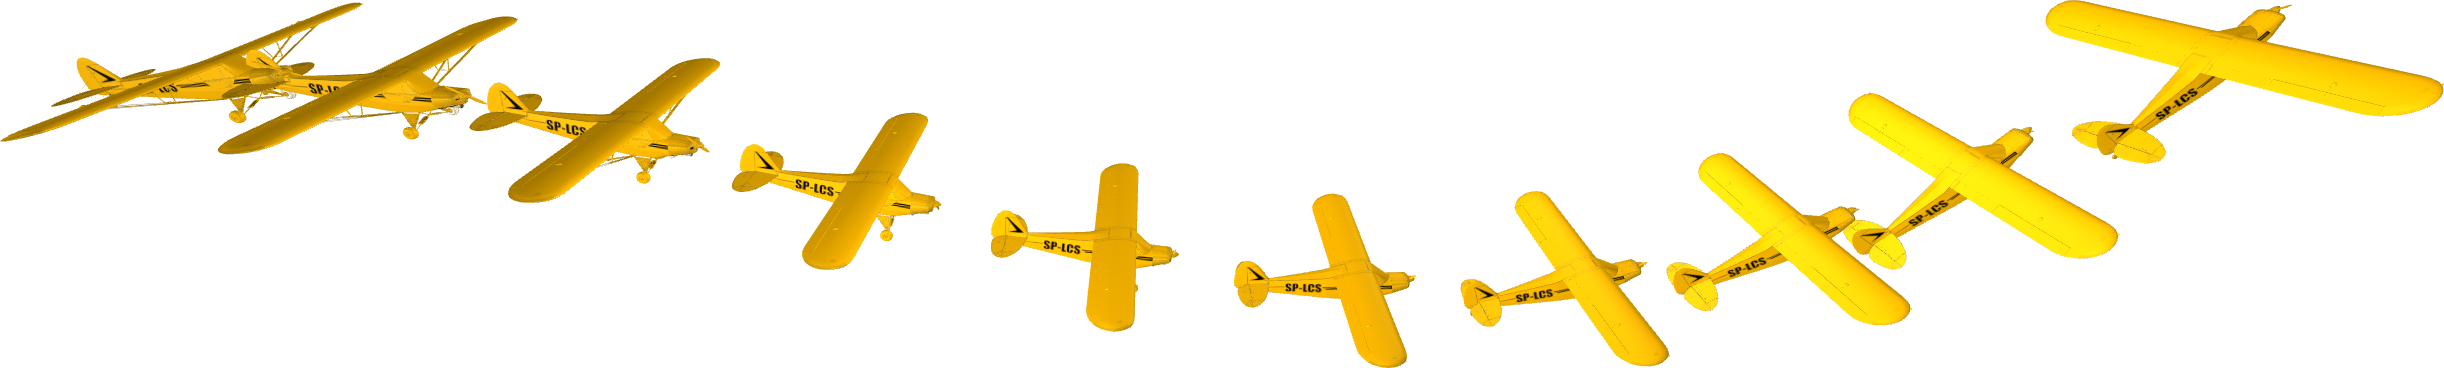
\includegraphics[width=\textwidth]{perch_cropped.png}
  \caption{Airplane perching trajectory, a high angle-of-attack maneuver that minimizes 
    velocity at the goal position}
  \label{fig:perch}
\end{figure}


%%%%%%%%%%%%%%%%%%%%%%%%%%%%%%%%%%%%%%%%%%%%%%%%%%%%%%%%%%%%%%%%%%%%%%%%%%%%%%%%%%%%%%%%%%
% Results
%%%%%%%%%%%%%%%%%%%%%%%%%%%%%%%%%%%%%%%%%%%%%%%%%%%%%%%%%%%%%%%%%%%%%%%%%%%%%%%%%%%%%%%%%%
\section{Results} \label{sec:results}

The following sections provide various numerical analyses of the proposed algorithm.  In
lieu of an actual hardware experiment (left for future work), for each simulated system we
specify two models: a \textit{nominal} model which is a simplified model approximating the
\textit{true} model, which contains both parametric and non-parametric model error from
the nominal model. This true model is used exclusively for simulating the system.

All models were trained by simulating the ``true'' system with an arbitrary controller to 
collect data in the region of the state space relevant to the task. A set of fixed-length 
trajectories were collected, each at a sample rate of 20 Hz. The bilinear eDMD model was
trained using the same approach introduced by Folkestad and Burdick \cite{Folkestad2021}.
All continuous dynamics were discretized with an explicit
fourth-order Runge Kutta integrator. 
We organize the following results section by topic, we briefly describe the three simulated
models used to produce the results in the paragraphs below.

The \textit{true} cartpole model included a $\tanh$ model of Coulomb friction between
the cart and the floor, viscous damping at both joints, and a control dead band that was not
included in the \textit{nominal} model. Additionally, the mass of the cart and pole model
were altered by 20\% and 25\% with respect to the nominal model, respectively.  The
following nonlinear mapping was used when learning the bilinear models: 
$\phi(x) = [\, 1,\,
x,\, \sin(x),\, \cos(x),\, \sin(2x),\, \sin(4x),\, T_2(x),\, T_3(x),\, T_4(x)\, ] \in
\R^{33}$, where $T_i(x)$ is a Chebyshev polynomial of the first kind of order $i$. 
All reference trajectories for the swing up task were generated using ALTRO 
\cite{Howell2019,Jackson2021}.

We also include 2 quadrotor systems: a 3-DOF, planar model and a 6-DOF, full quadrotor model. For both systems,
the \textit{true} model includes aerodynamic drag terms not included in the \textit{nominal} model, as well as parametric error of about 5\% on the system properties (e.g. mass, rotor arm length, etc.). The planar model was trained using a nonlinear mapping of $\phi(x) = [\, 1,\, x,\, \sin(x),\, \cos(x),\, \sin(2x),\, T_2(x) ] \in \R^{25}$ while the full quadrotor model was train using a nonlinear mapping of $\phi(x) = [\, 1,\, x,\, T_2(x),\, \sin(p),\, \cos(p),\, R^{T}v,\ v^{T}RR^{T}v,\, p \times v,\, p \times \omega,\, \omega \times \omega ] \in \R^{44}$, where $p$ is the quadrotor's position, $v$ and $\omega$ are the translational and angular velocities respectively, and $R$ is the Rotation matrix. Reference trajectories were produced by nominal MPC tracking controllers attempting to track infeasible, point-to-point, linear trajectories with various initial conditions.

Our most high-fidelity model is an airplane model with lift and drag coefficients fit from
rigorous wind-tunnel testing \cite{Manchester2017}. The coefficients are valid for high
angle-of-attach maneuvers. We produce a high-angle-of-attack (up to $40^\circ$) manuever by
solving for ``perching'' trajectories with ALTRO that encourage minimal velocity subject to
a constraint on the final position (see Figure \ref{fig:perch}). These trajectories are
tracked using a QP-based linear MPC solver, with bounds on the state and control deviations
at each time step. The nominal model used a simple flat-plate wing model with linear lift
and quadratic drag coefficient models. To train the bilinear models, we used a
68-dimensional nonlinear mapping composed of dynamics terms such as the rotation matrix
(expressed in terms of a Modified Rodriguez Parameter), powers of the angle of attack and
side slip angle, the body frame velocity, various cross products with the angular velocity,
and some 3rd and 4th order Chebyshev polynomials.

% nonlinear mapping: $\phi(x) = [1, x, \text{vec}(R), v_\text{body}, v_\text{body}^T
% v_\text{body}, \sin(p), \alpha, \beta, \alpha^2, \beta^2, \alpha^3, \beta^3, p \times v, p
% \times \omega, \omega \times \omega, T_3(x), T_4(x) ] \in \R^{68}$, where $p \in \R^3$ is
% the position, $g \in \R^3$ is the attitude expressed as Modified Rodriguez Parameter, $v \in
% \R^3$ is the linear velocity in the world frame, $\omega \in \R^3$ is the angular velocity,
% $R \in \R^{3 \times 3}$ is the rotation matrix expressed in terms of $g$, $v_\text{body}$ is
% the velocity in the body frame, $\alpha$ is the angle of attack, and $\beta$ is the side
% slip angle.

The code for the experiments is located at \todo{include after review}.  


%%%%%%%%%%%%%%%%%%%%%%%%%%%%%%%%%%%%%%%%%%%%%
\subsection{Sample Efficiency}
%%%%%%%%%%%%%%%%%%%%%%%%%%%%%%%%%%%%%%%%%%%%%
\begin{figure}[t]
  \centering
  \begin{subfigure}[t]{0.48\textwidth}
    \includegraphics[width=\textwidth, height=5cm]{../images/cartpole_mpc_test_error.tikz}
    % \includegraphics[width=\textwidth, height=5cm]{combined_mpc_test_error.tikz}
    \caption{Cartpole}
    \label{fig:cartpole_mpc_test_error}
  \end{subfigure}
  \hfill
  \begin{subfigure}[t]{0.48\textwidth}
    % \includegraphics[width=\textwidth, height=5cm]{rex_planar_quadrotor_mpc_test_error.tikz}
    \includegraphics[width=\textwidth,height=5cm]{airplane_error_by_num_train.tikz}
    \caption{Airplane}
    % \label{fig:planar_quad_mpc_test_error}
    % \includegraphics[width=\textwidth, height=5cm]{cartpole_mpc_train_time.tikz}
    % \caption{Training time for cartpole models as a function of training samples, using a 
    % preliminary implementation of the algorithm described in Section \ref{sec:rls}. The 
    % training time complexity is approximately linear.}
    % \label{fig:cartpole_train_time}
  \end{subfigure}
  \caption{MPC tracking error vs training trajectories for both the cartpole (left) and
  airplane (right). Tracking error is defined as the average L2 error over all the
  test trajectories between the reference and simulated trajectories.}
  \label{fig:sample_efficiency}
\end{figure}

We highlight the sample efficiency of the proposed algorithm in Figure 
\ref{fig:sample_efficiency}. For both the cartpole swing up and the airplane perch trajectory 
tracking tasks, the proposed method achieves better tracking than the nominal MPC controller
with just two sample trajectories, and performs uniformly better than eDMD on both 
trajectory tracking tasks. To achieve comparable performance on the perching task, eDMD 
requires about 4x the number of samples (20 vs 5) compared to the proposed approach.
\todo{add lines for ``lifted'' MPC approach?}


%%%%%%%%%%%%%%%%%%%%%%%%%%%%%%%%%%%%%%%%%%%%%
\subsection{Generalization}
%%%%%%%%%%%%%%%%%%%%%%%%%%%%%%%%%%%%%%%%%%%%%
\begin{figure}[t] \centering
  \begin{subfigure}[t]{0.49\textwidth}
    \centering
    \includegraphics[width=\textwidth,height=5cm]{rex_planar_quadrotor_lqr_error_by_equilibrium_change.tikz}
    \caption{LQR stabilization error over increasing equilibrium offset}
    \label{fig:rex_planar_quadrotor_lqr_error_by_equilibrium_change}
  \end{subfigure}
  \hfill
  \begin{subfigure}[t]{0.48\textwidth}
    \raggedright
    \includegraphics[width=\textwidth, height=5cm]{rex_planar_quadrotor_mpc_error_by_training_window.tikz}
    \caption{Tracking error for the quadrotor MPC reference trajectory tracking task.}
    \label{fig:rex_planar_quadrotor_mpc_error_by_training_window}
    % \includegraphics[width=\textwidth,height=5cm]{rex_planar_quadrotor_lqr_error_by_training_window.tikz}
    % \caption{Stabilization error for the quadrotor LQR stabilization task}
    % \label{fig:rex_planar_quadrotor_lqr_error_by_training_window}
  \end{subfigure}
  \caption{Generalizability with respect to initial conditions sampled outside of the 
  training domain. The initial conditions are sampled from a uniform distribution, whose 
  limits are determined by a scaling of the limits used for the training distribution. 
  A training range fraction greater than $1$ indicates the
  distribution range is beyond that used to generate the training trajectories. The thick 
  lines represent the algorithm with a heavy regularization parameter.
  }
  \label{fig:training_window}
\end{figure}


We demonstrate the generalizability of the proposed method to tasks outside of its training
domain in Figure \ref{fig:training_window}. In both the planar quadrotor 
stabilization (Figure \ref{fig:rex_planar_quadrotor_lqr_error_by_equilibrium_change}) and 
trajectory tracking (Figure \ref{fig:rex_planar_quadrotor_mpc_error_by_training_window})
tasks, we trained the models by sampling uniformly from a given window of offsets, centered 
about the origin. 
To test the generalizability of the methods we increased the relative size of the window 
from which the test data was sampled, e.g. if the initial lateral position was trained on 
data in the interval $[-1.5,+1.5]$, we sampled the test initial condition from the window 
$[-\gamma 1.5, +\gamma 1.5]$. As shown in the results, while the performance of the proposed
algorithm remains relatively constant even when $\gamma = 2.5$, whereas the classic eDMD 
approach looses performance and fails to generalize at all for the stabilization task using 
and LQR controller (like due to poor derivative information), and up to $\gamma = 2$ for the 
tracking task using a linear MPC controller.

In Figure \ref{fig:rex_planar_quadrotor_lqr_error_by_equilibrium_change} we show the effect 
of changing the equilibrium position for the planar quadrotor, but keeping the delta initial
conditions within the training window. As shown, eDMD doesn't generalize to other
equilibrium points, despite the fact that the underlying dynamics are invariant to the
equilibrium position. Our proposed approach, however, easily learns this from the derivative
information provided by the nominal model.

\begin{wraptable}{l}{9.0cm}
	\vspace{-2\baselineskip}
	\begin{tabular}{cccc}\\
		\toprule  
								& {\color{black} \textbf{nominal MPC}} & {\color{orange} \textbf{eDMD}} & {\textbf{\color{cyan} jDMD}} \\
		\midrule
		Mean Tracking Err.		& 0.30			& 0.63 	& \textbf{0.11} \\
		Success Rate 			& \textbf{82\%} & 18\%	& 80\% \\
		\bottomrule
	\end{tabular}
	\caption{Performance summary of MPC tracking of 6-DOF quadrotor}
	\vspace{-1\baselineskip}
	\label{tab:full_quad_tracking_mpc}
\end{wraptable} 

To demonstrate that this generalizability extends to more complex dynamics, we additionally 
show the tracking capabilities of infeasible, point-to-point trajectories for the 6-DOF quadrotor
with full attitude dynamics. As seen in Figure \ref{fig:rex_full_quadrotor_initial_conditions}, the generated
reference trajectories have a wide scope in sampling despite being sparse in nature. As shown in
Table \ref{tab:mpc_comp}, jDMD has the best tracking performance and closely matches nominal MPC's ability to
successfully reach the equilibrium. Meanwhile, eDMD has significantly worse performance in tracking and succeeding
in stabilizing about the goal state.  Despite the aggressive starting state, jDMD is still able to successfully
account for the attitude dynamics, reach the goal state, and stabilize, as seen in Figure \ref{fig:jdmd_full_quad_pointtopoint_with_waypoints}.

\begin{figure}[t] \centering
	\begin{subfigure}[t]{0.49\textwidth}
		\centering
		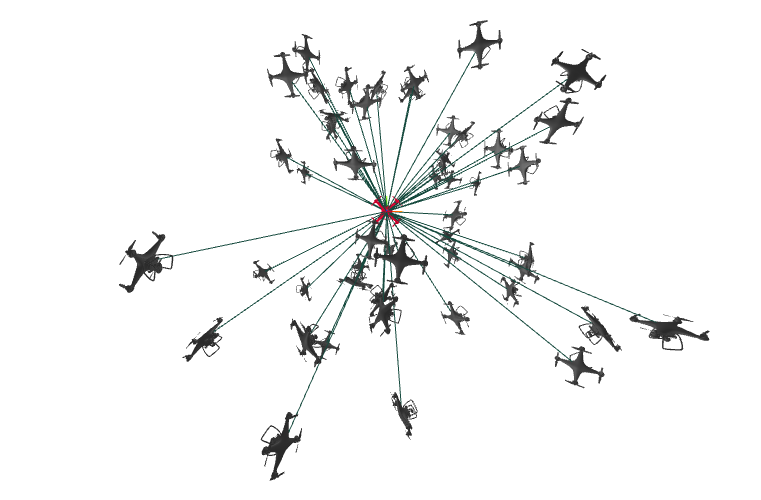
\includegraphics[width=\textwidth,height=5cm]{full_quadrotor_test_linear_trajectories.png}
		\caption{Generated point-to-point trajectories and initial conditions for testing tracking MPC of 6-DOF quadrotor.}
		\label{fig:rex_full_quadrotor_initial_conditions}
	\end{subfigure}
	\hfill
	\begin{subfigure}[t]{0.49\textwidth}
		\raggedright
		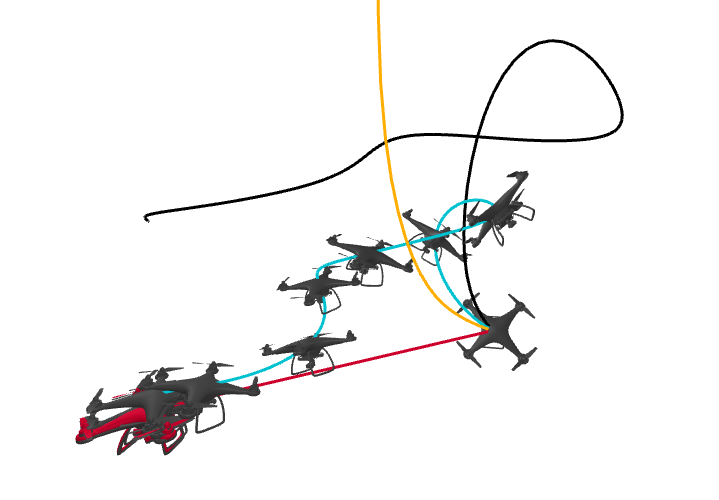
\includegraphics[width=\textwidth, height=5cm]{jdmd_full_quad_pointtopoint_with_waypoints.png}
		\caption{Generated MPC trajectories for nominal MPC (black), eDMD (\color{orange} orange\color{black}), and jDMD (\color{cyan} cyan\color{black})
    for tracking infeasible, point-to-point trajectory (\color{red} red\color{black}).}
		\label{fig:jdmd_full_quad_pointtopoint_with_waypoints}
		% \includegraphics[width=\textwidth,height=5cm]{rex_planar_quadrotor_lqr_error_by_training_window.tikz}
		% \label{fig:rex_planar_quadrotor_lqr_error_by_training_window}
	\end{subfigure}
	\caption{Generalizability with respect to initial conditions sampled outside of the 
		training domain. The initial conditions are sampled from a uniform distribution, whose 
		limits are determined by a scaling of the limits used for the training distribution. 
		A training range fraction greater than $1$ indicates the
		distribution range is beyond that used to generate the training trajectories. The thick 
		lines represent the algorithm with a heavy regularization parameter.
	}
	\label{fig:training_window}
\end{figure}

%%%%%%%%%%%%%%%%%%%%%%%%%%%%%%%%%%%%%%%%%%%%%
\subsection{Lifted versus Projected MPC}
%%%%%%%%%%%%%%%%%%%%%%%%%%%%%%%%%%%%%%%%%%%%%
\begin{wraptable}{r}{5.0cm}
  \vspace{-2\baselineskip}
  \begin{tabular}{ccc}\\
    \toprule  
    MPC       & {\color{orange} \textbf{eDMD}} & {\textbf{\color{cyan} jDMD}} \\
    \midrule
    Lifted    & 17   &          15 \\
    Projected & 18   &  \textbf{2} \\
    \bottomrule
  \end{tabular}
  \caption{Training trajectories required to beat nominal MPC}
  \vspace{-1\baselineskip}
  \label{tab:mpc_comp}
\end{wraptable} 
      
We performed a simple experiment to highlight the value of the proposed ``projected'' MPC,
outlined in \label{sec:projected_mpc}. We trained eDMD and jDMD models with an increasing 
number of training trajectories, and recorded the first sample size at which the ``lifted''
and ``projected'' MPC controllers consistently stabilized the system (i.e. stabilized 95\%
of the test initial conditions for the cartpole system for that sample size and subsequent 
ones). The results are summarized in Table \ref{tab:mpc_comp}. The results qualitatively 
show what we quantitatively observed while training and testing these various examples:
the projected MPC approach usually required far fewer samples to ``train'' and usually had 
better performance than it's ``lifted'' counterpart that used the bilinear ``lifted'' 
dynamics. This was especially pronounced when combined with the proposed jDMD approach, 
which makes sense given that the approach explicitly encourages these Jacobians to match 
the analytical ones, so quickly converge to reasonable values with just a few training 
examples.

\subsection{Sensitivity to Model Mismatch}

While we've introduced a significant mount of model mismatch in all of the examples so far,
a natural argument against model-based methods is that they're only as good as your model is
at capturing the salient dynamics of the system.  We investigated the effect of increasing
model mismatch by incrementally increasing the Coulomb friction coefficient between the cart
and the floor for the cartpole stabilization task (recall the nominal model assumed zero
friction). The results are shown in Figure \ref{tab:friction_comp}. As expected, the number
of training trajectories required to find a good stabilizing controller increases for the
proposed approach. We achieved the results above by setting $\alpha = 0.01$, corresponding 
to a decreased confidence in our model, thereby placing greater weight on the experimental 
data. The standard eDMD approach always required more samples, and was unable to find a good
enough model above friction values of 0.4. While this could likely be remedied by adjusting
the nonlinear mapping $\phi$, the proposed approach works well with the given bases.  Note
that the nominal MPC controller failed to stabilize the system above friction values of 0.1,
so again, we demonstrate that we can improve MPC performance substantially with just a few
training samples by combining analytical gradient information and data sampled from the true
dynamics.

\begin{table}[t]
  \centering
  \begin{tabular}{cccccccc}
  \toprule 
  Friction ($\mu$) & 0.0 & 0.1 & 0.2 & 0.3 & 0.4 & 0.5 & 0.6 \\
  \midrule 
  Nominal & \cmark & \cmark & \xmark & \xmark & \xmark & \xmark & \xmark \\
  eDMD & 3 & 19 & 6 & 14 & \xmark & \xmark & \xmark \\
  jDMD & 2 & 2 & 2 & 2 & 3 & 7 & 12 \\
  \end{tabular}
  % \include(../images/tables/friction_comp.tex)
  \caption{Training trajectories required to stabilize the cartpole with the given friction
    coefficient
  }
  \label{tab:friction_comp}
\end{table}


%%%%%%%%%%%%%%%%%%%%%%%%%%%%%%%%%%%%%%%%%%%%%%%%%%%%%%%%%%%%%%%%%%%%%%%%%%%%%%%%%%%%%%%%%%
% Limitations 
%%%%%%%%%%%%%%%%%%%%%%%%%%%%%%%%%%%%%%%%%%%%%%%%%%%%%%%%%%%%%%%%%%%%%%%%%%%%%%%%%%%%%%%%%%
\section{Limitations} \label{sec:limitations}
As with most data-driven techniques, it is hard to definitively declare that the proposed 
method will increase performance in all cases. It is possible that having an extremely poor
analytical model may hurt rather than help the training process. However, we found that even
when the $\alpha$ parameter is extremely small (placing little weight on the Jacobians 
during the learning process), it still dramatically improves the sample efficiency. It is 
also quite possible that the performance gaps between eDMD and jDMD shown here can be 
reduced through better selection of basis functions and better training data sets; however,
given that the proposed approach converges to eDMD as $\alpha \rightarrow 0$, we see no 
reason to not adopt the proposed methodology as simply tune $\alpha$ based on the 
confidence of the model and the quantity (and quality) of training data.


%%%%%%%%%%%%%%%%%%%%%%%%%%%%%%%%%%%%%%%%%%%%%%%%%%%%%%%%%%%%%%%%%%%%%%%%%%%%%%%%%%%%%%%%%%
% Conclusion 
%%%%%%%%%%%%%%%%%%%%%%%%%%%%%%%%%%%%%%%%%%%%%%%%%%%%%%%%%%%%%%%%%%%%%%%%%%%%%%%%%%%%%%%%%%
\section{Conclusion and Future Work} \label{sec:conclusion}

We have presented a simple but powerful extension to eDMD, a model-based method for learning
a bilinear representation of arbitrary dynamical systems, that incorporates derivative
information from an analytical model. When combined with a simple linear MPC policy that
projects the learned dynamics back into the original state space, we have shown that the
resulting pipeline can dramatically increase sample efficiency, often improving over a
nominal MPC policy with just a few sample trajectories. Substantial areas for future work
remain: most notably testing the proposed pipeline on hardware. Additional directions
include lifelong learning or adaptive control applications, combining simulated and real
data through the use of modern differentiable physics engines \cite{Howell2022,Todorov2012}
residual dynamics learning, as well as the development of specialized numerical methods for
solving nonlinear optimal control problems using the learned bilinear dynamics.

\bibliography{Koopman.bib}

\end{document}
